\documentclass[11pt]{EuclidVIS}
\usepackage[utf8]{inputenc}
\usepackage[english]{babel}
\usepackage[top=1.9cm, bottom=5.4 cm, left=2.5cm, right=2.5cm]{geometry} 
\usepackage{amsmath}
\usepackage{amssymb}
\usepackage{amsfonts}
\usepackage{graphicx}
\usepackage{fancyhdr}
\usepackage{multirow}
\usepackage{tabularx}
\usepackage{subcaption}
\usepackage{lastpage}
\usepackage[usenames, dvipsnames, svgnames, table]{xcolor} 
\usepackage[nodayofweek]{datetime}
\usepackage{pbox}
\usepackage[titletoc]{appendix}
\usepackage[labelfont={color=MidnightBlue,bf}, textfont={color=MidnightBlue}]{caption}
\usepackage{appendix}
\usepackage{gensymb}
%
% UPDATE YOUR NAME HERE
%
\usepackage[pdfauthor={Marco C Lam}, bookmarks=true, colorlinks=true, linktoc=section, linkcolor=black]{hyperref} 
\usepackage{tocloft} 
\usepackage[ulem=normalem]{changes} 
\usepackage{pifont}
\usepackage{natbib}
\usepackage{url}
\usepackage{tikz}
\usetikzlibrary{positioning, decorations.pathreplacing, calc, arrows.meta, shapes.geometric}


\newcommand{\la}{\,\rlap{\raise 0.5ex\hbox{$<$}}{\lower 1.0ex\hbox{$\sim$}}\,}
\newcommand{\ga}{\,\rlap{\raise 0.5ex\hbox{$>$}}{\lower 1.0ex\hbox{$\sim$}}\,}

\def\vec#1{\ensuremath{\mathchoice{\mbox{\boldmath$\displaystyle#1$}}
{\mbox{\boldmath$\textstyle#1$}}
{\mbox{\boldmath$\scriptstyle#1$}}
{\mbox{\boldmath$\scriptscriptstyle#1$}}}}
%
\def\tens#1{\ensuremath{\mathsf{#1}}}

\def\i{{\rm{i}}}
\def\L{\log\mathcal{L}}

\input{refs}


%change tracking:
% - use latexdiff 
% - use the changes package


%SMN settings
\newcommand{\gresim}{\ {\raise-.5ex\hbox{$\buildrel>\over\sim$}}\ }
\newcommand{\lessim}{\ {\raise-.5ex\hbox{$\buildrel<\over\sim$}}\ }
\def\degC{$^\circ\kern-0.06em\rm{C}$} %Celsius

%Section number to table and figure
\numberwithin{table}{section}
\numberwithin{figure}{section}

%Table padding
\newcommand\T{\rule{0pt}{4ex}}       % Top strut
\newcommand\B{\rule[-3ex]{0pt}{0pt}} % Bottom strut

%to fix the gray page numbers in the ToC
\makeatletter
\let\stdl@section\l@section
\renewcommand*{\l@section}[2]{%
  \stdl@section{\textcolor{black}{#1}}{\textcolor{black}{#2}}}
\let\stdl@subsection\l@subsection
\renewcommand*{\l@subsection}[2]{%
  \stdl@subsection{\textcolor{black}{#1}}{\textcolor{black}{#2}}}
\makeatother

%cite label
\makeatletter
\newcommand{\customlabel}[2]{%
\protected@write \@auxout {}{\string \newlabel {#1}{{#2}{}}}}
\makeatother


%header mods
\setlength{\headheight}{72pt}
\pagestyle{fancy}\fancyhf{}
\renewcommand{\headrulewidth}{0pt} 

%footnotes
\renewcommand{\thefootnote}{\fnsymbol{footnote}}

%date mods
\renewcommand{\dateseparator}{/}
\newcommand{\todayiso}{\twodigit\day \dateseparator \twodigit\month \dateseparator \the\year}

%table mods
\renewcommand{\arraystretch}{1.1}

%margin notes
\newcommand{\cross}{\ding{55}}
\newcommand{\mused}{\marginpar[\hfill \huge \checkmark]{\huge \checkmark}}
\newcommand{\mprob}{\marginpar[\Huge \bf !]{\hfill \Huge \bf !}}
\newcommand{\mokay}{\marginpar[\Huge \tick]{\hfill \Huge \tick}}
\newcommand{\mbad}{\marginpar[\Huge \cross]{\hfill \Huge \cross}}


%-------------------------------------------------------------------------------
%	HEADER INFORMATION
%-------------------------------------------------------------------------------
\definecolor{light-gray}{gray}{0.5}

\fancyhead[C]{
    \color{light-gray}{
        \begin{tabular}{| l | c | r | l |}
        \hline
        \multirow{4}{*}{
\includegraphics[width=2cm]{logo.png}} % LOGO
        %\multirow{4}{*}{\Huge{EC}} % LOGO
        &\multirow{4}{*}{\pbox{7.5cm}{\Large{SHE Sensitivity Testing}}}
        &\textbf{Ref.:} & EUCL-EDI-TN-?-??? \\
        &&\textbf{Issue:} & 1.0 \\ 
%        &&\textbf{Date:} & 16$^{\rm th}$\,July 2024 \\ 
        &&\textbf{Date:} & \today \\ 
        &&\textbf{Page:} & \thepage/{\hypersetup{linkcolor=light-gray}\pageref{LastPage}} \\
        \hline
        \end{tabular}
    }
}
%-------------------------------------------------------------------------------
%	FOOTER INFORMATION
%-------------------------------------------------------------------------------
%\renewcommand{\footrulewidth}{0.0pt}
\fancyfoot[C]{\footnotesize{\color{light-gray}{
The presented document is Proprietary information of the Euclid Consortium.
This document shall be used and disclosed by the receiving Party and its
related entities (e.g. contractors and subcontractors) only for the purposes of
fulfilling the receiving Party's responsibilities under the Euclid Project and
that the identified and marked technical data shall not be disclosed or
retransferred to any other entity without prior written permission of the
document preparer.}}}

\begin{document}
\color{black}

%-------------------------------------------------------------------------------
%   FRONT PAGE
%-------------------------------------------------------------------------------

\section*{}
\vspace{+0.2cm}
\noindent
\begin{tabularx}{1.0\textwidth}{ | r | X | r | l |}
\hline
\textbf{Title:} & SHE Sensitivity Test & & \\
\hline
\textbf{Date:} & \today & \textbf{Issue:} & 1.0 \\
\hline
\textbf{Reference:} & EUCL-EDI-TN-?-??? & & \\
\hline
\textbf{Custodian:} & Marco C Lam & Edinburgh &\\
\hline
\end{tabularx}


\vspace{+4cm}
\noindent
\begin{tabularx}{1.0\textwidth}{ | l | X | c | l |}
\hline
\rowcolor{gray!30}
\textbf{Authors:} & \textbf{Position:} & \textbf{Date:} & \textbf{Signature:}\\
\hline
%Marco C Lam & University of Edinburgh & 28 June 2024 & \\
Marco C Lam & University of Edinburgh & \today & \\
\hline
\rowcolor{gray!30}
\textbf{Contributors:} & & & \\
\hline
%Ian Fenech Conti & University of Malta & & \\
%Edo van Uitert & University College London & & \\
%J\'{e}r\^{o}me Amiaux & CEA Saclay \\
%Pierre-Antoine Frugier & CEA Saclay & & \\
%Samuel Ronayette & CEA Saclay & & \\
%Koryo Okumura & CEA Saclay & & \\
%Julien Merten & University of Oxford & & \\
%Corentin Schreiber & University of Oxford & & \\
%Imogen Whittam & University of Oxford & & \\
%Martyn Wells & ATC Edinburgh & & \\
%Alessio Magro & University of Malta && \\
%Tobias Boenke & ESA && \\
\hline
\rowcolor{gray!30}
\textbf{Approved by:} & & &\\
\hline
&&&\\
\hline
\rowcolor{gray!30}
\textbf{Authorised by:} & & &\\
\hline
&&&\\
\hline
\end{tabularx}

\newpage


%-------------------------------------------------------------------------------
% TRACKING
%-------------------------------------------------------------------------------

\section*{}
\section*{\center{Document version tracking}}

\vspace{+0.3cm}
\noindent
\begin{tabularx}{1.0\textwidth}{ | c | c | c | X | l |}
\hline
\rowcolor{gray!30}
\textbf{Issue} & \textbf{Date} & \textbf{Pages} & \textbf{Description of Change} & \textbf{Comments}\\
\hline
1.0 & 29/11/2023 & All & New Document & Initial Draft \\
\hline
\end{tabularx}

\newpage

%-------------------------------------------------------------------------------
% TOC
%-------------------------------------------------------------------------------

\renewcommand*{\contentsname}{\color{MidnightBlue}{Table of Contents}}
\setcounter{tocdepth}{3}
\setlength{\cftbeforetoctitleskip}{-1em}
\cftsetindents{section}{0em}{1.5em}
\cftsetindents{subsection}{1.5em}{2em}
\cftsetindents{subsubsection}{4em}{2em}
\tableofcontents
\addtocontents{toc}{\vskip-20pt} 
\thispagestyle{fancy}

%-------------------------------------------------------------------------------
% Purpose and Scope
%-------------------------------------------------------------------------------
\newpage

\section*{Purpose}
This document presents the motivation, methodology, and results of the
Sensitivity Testing programme run within OU-SHE. This programme investigates
the sensitivity of various shear estimation methods and galaxy properties'
effects on shape measurement. This assesses the bias on the shear measurements,
ensuring the expected measurement uncertainties of these properties will not
exceed the requirements defined by the \textit{Euclid} mission.

\section*{Scope}
Talk about the scope

\newpage


%-------------------------------------------------------------------------------
% Applicable and Reference Documents
%-------------------------------------------------------------------------------

\section*{Applicable \& Reference Documents}

\subsection{Applicable Documents}

\noindent
\begin{tabularx}{1.0\textwidth}{ | l | X | X | r |}
\hline
\rowcolor{gray!30}
\textbf{AD} & \textbf{Title} & \textbf{Reference} & \textbf{Date}\\
AD1 & SGS VIS PSF model generation & EUCL-OXF-TN-8-001 issue 2 & 1/10/2020 \\
\hline
AD2 & Euclid Science Requirements Document (SciRD) & EUCL-EST-RQ-9-001 issue 7 & 25/08/2015 \\
\hline
AD2 & Euclid Ground Data Processing Requirements Document & EUCL-EST-RS-8-001 issue 3 & 20/10/2014 \\
\hline
\end{tabularx}


%\vspace{+1cm}
\begingroup
\subsection{Reference Documents}
\let\clearpage\relax %remove new page
\vspace*{-3cm}
\renewcommand{\bibname}{}
\bibliographystyle{plainnat}
\bibliography{references}
\endgroup

%TODO: write this so that referencing works...

%\makeatletter
%\renewenvironment{thebibliography}[1]
%     {\begin{multicols}{3}[]%
%      \@mkboth{\MakeUppercase\refname}{\MakeUppercase\refname}%
%      \list{\@biblabel{\@arabic\c@enumiv}}%
%           {\settowidth\labelwidth{\@biblabel{#1}}%
%            \leftmargin\labelwidth
%            \advance\leftmargin\labelsep
%            \@openbib@code
%            \usecounter{enumiv}%
%            \let\p@enumiv\@empty
%            \renewcommand\theenumiv{\@arabic\c@enumiv}}%
%      \sloppy
%      \clubpenalty4000
%      \@clubpenalty \clubpenalty
%      \widowpenalty4000%
%      \sfcode`\.\@m}
%     {\def\@noitemerr
%       {\@latex@warning{Empty `thebibliography' environment}}%
%      \endlist\end{multicols}}
%\makeatother

%\renewcommand\bibname{} %remove name
%\let\clearpage\relax %remove new page
%\begin{thebibliography}{}
% \bibitem[AD1]{ref1}{A.N. Other \& S.O.M. Ebody}{eucl-mssl-xxx-yyyy-}{09/2010}
% \bibitem[AD2]{ref2}{author}{eucl-mssl-xxx-yyyy-}{09/2012}
%\end{thebibliography}

%\noindent
%\begin{tabularx}{1.0\textwidth}{ | l | X | c | c |}
%\hline
%\rowcolor{gray!30}
%\textbf{RD} & \textbf{Title} & \textbf{Reference} & \textbf{Date}\\
% & & & \\
%\hline
%&&& \\
%\hline
%\end{tabularx}

\newpage


%-------------------------------------------------------------------------------
% Accronyms
%-------------------------------------------------------------------------------

\section*{Acronyms}

\begin{tabular}{l l}
%ACS & HST Advanced Camera for Surveys \\
%ADS & Airbus Defence and Space \\  
%AOCS & Attitude and Orbit Control System \\  
%AoI & Angle of Incidence \\
%BFE & Brighter-Fatter Effect \\
CCD & Charge Coupled Device \\
%CDR & Comprehensive Design Review \\
%{\sc codeen} & (SGS) Collaborative Development Environment \\
%CTI & Charge Transfer Inefficiency \\
DET & DETector  (only for referring to VIS DET data)\\
%FD & Fourier Domain \\
FoV & Field of View \\
%FFT & Fast Fourier Transform \\
%FGS & Fine Guidance Sensor \\
%FOM\,(1,2,3) & Fold Mirror (1,2 or 3) \\
%FM & Flight Module \\
%FS & Fight Spare \\
%GDPRD & Ground Data Processing Requirements Document \\
%HST & Hubble Space Telescope\\
%M1  & Primary Mirror \\
%M2  & Secondary Mirror\\
%M3  & Tertiary Mirror \\
%MDB & Mission DataBase \\
%MPI & Message Passing Interface \\
%OPD & Optical Path Difference \\
%PDR & Preliminary Design Review \\
%PLM & Payload Module \\
%PRNU & Photo Response Non-Uniformity \\
%PSD & Power Spectral Density \\
PSF & Point Spread Function\\
%RPE & Relative Pointing Error \\
%RSD & Reference Survey Design \\
%RSU & Readout Shutter Unit \\
%SAA & Solar Aspect Angle \\
%SciRD & Science Requirements Document \\
SDC & Science Data Centre \\
SED & Spectral Energy Distribution \\
%SFE & Surface Figure Error \\
SGS & Science Ground Segment \\
%SNR & Signal-to-Noise Ratio\\
%SOPS & Special Operations \\
%STOP & Structural-Thermal-Optical (analysis) \\
VIS & Visible Instrument \\
WCS & World Coordinate System \\
%WFE & Wavefront Error \\
\end{tabular}


\newpage

%---------------------------------------------------------------------------------------------------
% Article starts
%---------------------------------------------------------------------------------------------------
\section{Introduction}
\textit{Euclid} is designed to optimise its instrumentation and observing strategy for two
complementary methods, the weak gravitational lensing~(WL) method and the baryonic acoustic
oscillations~(BAO) method. Sensitivity testing regards the systematics in the galaxy shape
measurement methods used by the WL method. These sysmatics can be found from repeating observation
with known input configurations. However, it is not possible to create new universes for
repeated observations; the only way forward is to rely on simulations to understand the shape
measurement methods.

%---------------------------------------------------------------------------------------------------
Everything in the data collection, reduction and analysis process can lead to a bias in the
measurement. However, some effects are much more dominant than others. \cite{2007MNRAS.376...13M}
and \cite{2013MNRAS.431.3103C} have extensively investigated the impact of various selection and
measurement properties that are necessary to achieve high-prevision weak-lensing analysis.
\cite{2017MNRAS.467.1627F} brought it further to understand how the biases in shape measurements
are as functions of various properties, and is now known as the \textit{sensitivity}. The process
of qualitatively defining the effects is \textit{sensitivity testing}.

%---------------------------------------------------------------------------------------------------
It is well understood that one of the most dominant source of bias is that from the point spread
function~(PSF; \citealp{2008A&A...484...67P, 2013MNRAS.429..661M}). Noise in the observations (or
in simulations) also plays an important part in biasing in shape measurements~(e.g.\ \citealp{2012MNRAS.424.2757M}),
to name a few, they can come from the random background noise, imperfect detector effect correction,
imperfect cosmic ray removal, unknown number density of faint background galaxies, colours of the
galaxy population and so on. These effects can be calibrated out using significant simulation effort,
such kind of calibration has demonstrated success in numerous works, for example, in the
Canada-France-Hawaii Telescope Lensing Survey~\citep{2013MNRAS.429.2858M}, the Hyper Suprime-Cam
Survey~\citep{2018MNRAS.481.3170M}, the Kilo-Degree Survey~\citep{2021A&A...645A.105G}, and the
Dark Energy Survey~\citep{2022MNRAS.509.3371M}.

%---------------------------------------------------------------------------------------------------
At the SDC-UK, the work package of \textit{Sensitivity Testing} consists of three main components:
(1)~\textit{Euclid} Visible Instrument~(VIS)-like image simulation; (2) shear measurement with
\textsc{LensMC} and \textsc{Metacal}, along with a direct \textsc{KSB} as
a consistency check; and (3) assess the change in the biases as functions of a range of variables.
This technical note is organised as follow: in Section~\ref{sec:definition_and_requirement}, we 
define the terms and high-level requirements; in Section~\ref{sec:simulation} and \ref{sec:shape_measurement},
we provide high-level description of the simulation and measurement methods. The detailed workflow
will be described in Section~\ref{sec:workflow}. The results for various sensitivity tests will
be presented in Section~\ref{sec:results}.

%---------------------------------------------------------------------------------------------------
\section{Definitions and Requirements}
\label{sec:definition_and_requirement}
%---------------------------------------------------------------------------------------------------
On the projected plane of observation, shear can be parameterised in two different forms, the $e$-
and $g$-conventions. While the shape measurement methods are categorically divided into two broad
types, one is based on moments measurement and the other on profile (template) fitting. All methods
have their own strength and drawback, hence the types and strength of the biases are all independent
for each method and most intermediate measurables are not directly comparable. This section defines
the terms and parameterisation of the shear estimates and underlying assumptions in our simulation.

%---------------------------------------------------------------------------------------------------
\subsection{Shear and Bias}
%---------------------------------------------------------------------------------------------------
For shear estimates, the \textit{Euclid} mission~\citep{2024arXiv240513491E} adopts the formalism of \cite{2020OJAp....3E..14K}
where the estimated shear~($\hat{\gamma}$) and true shear ($\gamma$) are complex numbers and their
difference can be expressed to first order
\begin{equation}
\label{eq:true_shear}
    \hat{\gamma} - \gamma = m_{0}^{\mathrm{bias}} \gamma + m_{4}^{\mathrm{bias}} \gamma^{*} + c^{\mathrm{bias}} + n 
\end{equation}
where $m_0$ and $m_4$ are the spin-0 and spin-4 complex operators (multiplicative bias), 
respectively; the asterisk denotes complex conjugation. The value of $m_0$ quantifies the dilation
and rotation of the true shear, whereas $m_4$ allows for a reflection around the axis determined by
its phase, $c$ is the additive bias, while n corresponds to the random statistical shape noise in 
the shear estimate.

%---------------------------------------------------------------------------------------------------
In this work, we only explore the sensitivity of the spin-0 multiplicative bias and we only concern 
the reduced shear, $g$, which is defined as $g = \frac{\gamma}{1 - \kappa}$, or $|g| = \frac{a-b}{a+b}$,
where $\kappa$ is the convergence, a negative $\kappa$ increases the size
of the source, a positive value reduces; $a$ is the semi-major axis and $b$ is the semi-minor axies.
Substitute this into Equation~\ref{eq:true_shear}, it simplifies to
\begin{equation}
    \mathbf{g}' = (1 + \mathbf{m}) \mathbf{g} + \mathbf{c}
\end{equation}
where $\mathbf{g}$ and $\mathbf{g}'$ are two-vectors that $g_1$ refers to stretching in the
orthogonal directions and $g_2$ is the same form of distortion along the axes rotated by 
$45^{\degree}$ to those of $g_1$~(see Figure~\ref{fig:kappag1g2}), $\mathbf{m}$ and $\mathbf{c}$ are
the multiplicative and addictive biases in the shear measurements. The effects of bias on the two
components of shear are assumed to be independent.

\begin{figure}
    \centering
    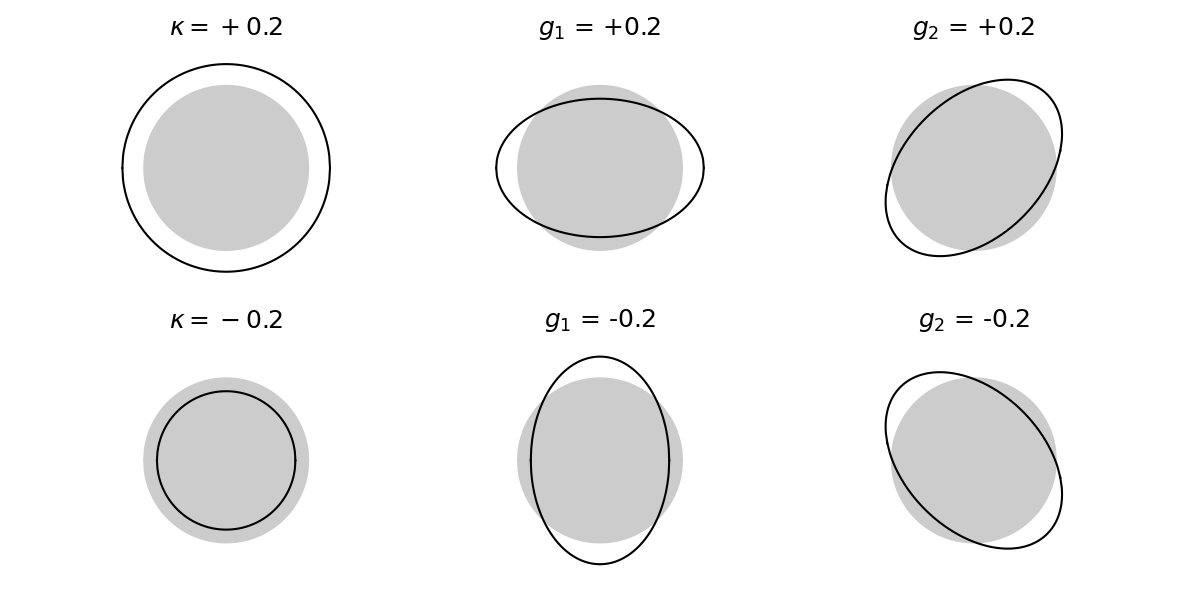
\includegraphics[width=\linewidth]{figures/kappa_g1_g2.png}
    \caption{Effect of the components of $\kappa$, $g_1$ and $g_2$ on a circular source
    represented by the solid grey circle. Black line shows the shapes of the respective sheared
    circular sources.}
    \label{fig:kappag1g2}
\end{figure}

Throughout SHE, despite the shapes measured are represented with the variables $e_1$ and $e_2$, which are the
\underline{e}llipticities of the galaxies, not to mix up with the $e$-convention of shear
description, where $|e|=\frac{a^2 - b^2}{a^2 + b^2}$. The directions in which $e_1$ modulates the
dilation and contraction are aligned with the equatorial coordinate system, where positive $e_1$ is
a dilation in the direction of Right Ascension~(RA) and contraction in the direction of Declination~(Dec),
and a positive $e_2$ dilates in the direction of $(-\mathrm{RA}, \mathrm{Dec})$.

%---------------------------------------------------------------------------------------------------
\subsection{Sensitivity}
%---------------------------------------------------------------------------------------------------
All things can lead to a bias in the shear measurement, but some properties have much stronger
effects than others. In many cases, the size of the bias is specific to the instrument, survey
strategy and measurement method, so results from previous works are not directly applicable to a
new survey. However, they formed the basis of an excellent preliminary list of parameters that
have to be investigated for their effects on shear measurements. The term \textit{sensitivity} is
used to describe how sensitive the change in the multiplicative bias ($\Delta m$)\footnote{sometimes
$\mu$ is used instead of $m$.} and the additive
bias ($\Delta c$) as a function of a given parameter. For instance, it can be the local sky
background level, the intrinsic distribution of the size of galaxies, the PSF model, etc.  This is
the most important in the preparation of the calibration effect that actually subtracts the biases
from the measurement. The significance of performing sensitivity tests is to understand which
properties need to be better understood and taken care of in the process of calibration.

%---------------------------------------------------------------------------------------------------
\subsection{Requirements}
%---------------------------------------------------------------------------------------------------
%Euclid Overview article \citep{2024arXiv240513491E}:
Various requirements would be relevant to this work; the most important one is the set that governs
the additive and multiplicative biases. From the Euclid Science Requirements Document (Issue 7,
Revision 1), \textbf{R-WL.2.1-24} has stated

\begin{quote}
    ``We require the multiplicative bias in shape measurement to be known to an accuracy of $\sigma_\mu \leq 2 \times 10^{-3}$ and the additive bias to be known to an accuracy of $\sigma_c \leq 5 \times 10^{-4}$ under all observing conditions and for all type of object used for weak lensing.''
\end{quote}

Sensitivity testing will allow us to understand the `operational range' of the shape measurement
methods -- the parameter space in which the methods deliver results within the requirements.
Other requirements (or quoted from the detailed descriptive text for the requirements,
\textbf{T}) this work will naturally validate the following:
\begin{enumerate}
    \item R-WL.1-2 ``The average density of galaxies over the survey area that are useful for weak gravitational lensing shall be $\geq30$ galaxies per arcmin$^2$.''
    \item R-WL.1-3 ``The redshift distribution of the lensed galaxies shall have a median redshift greater than 0.8.''
    \item T-WL.1-7 ``...a minimum of 10 tomographic bins... calibration sample will need to exceed $10^4$ galaxies...''
    \item R-WL.2.1-5 ``The ellipticity of the VIS PSF, measured from an image that has been exposed for the nominal integration time, shall be less than 0.15''.
\end{enumerate}

%---------------------------------------------------------------------------------------------------
\section{Simulation}
\label{sec:simulation}
%---------------------------------------------------------------------------------------------------
The simulation work starts with the output catalogue from the Flagship hydrodynamical simulation
and the True Universe star catalogues. We assume their simulated version of the Galaxy and the
Universe is realistic. The SHE Calibration working group tackles the issues arising from unrealism,
and it is beyond the scope of this work. Star-galaxy separation is perfect because we have the
ground truth from the input catalogues. The effect from contamination by stars on the biases is
beyond the scope of this work. Galaxies with visibly complex morphologies are also not included.
All galaxies follow inclined S{\'e}rsic surface brightness profiles containing a bulge component
and sometimes also a disk component. Intrinsic galaxy alignment is included in the Flagship
simulation, hence, it would be exhibited in our simulation.

All detector defects are not included, for example, there is no simulation on the charge transfer 
inefficiency, blooming, brighter-fatter effect, ghosting, stray-light, cross-talk, etc. Cosmic
rays and dead pixels are also not included.

%---------------------------------------------------------------------------------------------------
\subsection{VIS DET image}
%---------------------------------------------------------------------------------------------------
Constructing a realistic World Coordinate System~(WCS) for the 144 detector quadrants on the
focal plane requires tremendous effort. Realistically mocking up other header information is also
non-trivial. Because of that, as this project was started after launch, we use the data product of
the VISCalibratedQuadFrames as starting points of the simulation. The data product contains all the 
essential meta-information of the WCS and detector information to simulate a realistic image, given 
good input catalogues of stars and galaxies, and their spectral information~(see the next two 
subsections).

%---------------------------------------------------------------------------------------------------
\subsection{Stars}
%---------------------------------------------------------------------------------------------------
The stars in the image simulation are taken from the Star Catalogue prepared by the
\textit{Euclid}-SGS-SIM working group. The catalogue contains a selected coverage of the sky that
have made use of (1)~real data from Gaia DR3 catalogues for the brighter sources~($G <=
18.25\,\mathrm{mag}$); (2)~synthetic stars from the Besan\c{c}on Galaxy Model for sources fainter
than  $18.25\,\mathrm{mag}$; (3)~8680 BASeL spectra covering a sparsely populated grid at 69 
effective temperature~($\mathrm{T}_{\mathrm{eff}}$), 20 surface gravities~($\log(g)$), and 20
metallicities~([Fe/H]). The stellar density is appropriate for the given part of the sky, star 
clusters are not included, which makes it directly usable for our work. A comprehensive description
to the Star Catalogue should be referred to the wiki page on
Redmine~(\url{https://euclid.roe.ac.uk/projects/sim_trueuniverse/wiki/SPV3_TU_stars}). 
In the simulation, we include all the stars available from the catalogue. The data can be retrieved
from the Euclid DBView Web Service at \url{https://eas-dps-cus-ops.esac.esa.int}.

%---------------------------------------------------------------------------------------------------
\subsection{Galaxies}
%---------------------------------------------------------------------------------------------------
Flagship simulation~\citep{2024arXiv240513495E} is an N-body dark matter simulation with $16000^3$
particles. It is designed to support the scientific exploitation of the Euclid mission. It contains
a catalogue of 16 billion haloes in one octant of the sky in the lightcone up to redshift $z=3$.
Galaxies are then populated in these haloes using a halo occupation distribution and abundance 
matching approach, calibrating the free parameters of the galaxy mock against observed correlations
and other basic galaxy properties. A comprehensive set of galaxy properties are modelled for the 
final sample of 3.4 billion galaxies. Each galaxy is assigned with one of the 31 galaxy spectra. All
the necessary quantities for this work, for example, position, redshift, shear values, axis ratio,
S\'{e}rsic indices, spectral type are included. The catalogue can be queried along with the
auxiliary data at \url{https://cosmohub.pic.es/catalogs/298}.

%---------------------------------------------------------------------------------------------------
\subsection{Point Spread Functions}
%---------------------------------------------------------------------------------------------------
In order to render a simulated image, we need to convolve a point spread function~(PSF) with the 
sources. To do so, we use the \textsc{PSFToolkit} to generate a realistic VIS PSF for this work. VIS
has a field of view~(FoV) dimension of roughly $40' \times 40'$, spanning over 36 4k
detectors, each subdivided into four quadrants, giving a set of 144 ``images'' per exposure. 
Over such a large focal plane, PSF varies significantly with position. Thus, even for the purpose
of simulation, we are using a static set of monochromatic basis PSFs per-quadrant~(roughly $3.3`
\times 3.3`$). The PSF of a source is the sum of the basis set weighted by the spectral energy 
distribution~(SED) function. Fig.~\ref{fig:enter-label} illustrates how the PSF varies as a function
of SEDs (O, B, A, F, G, K \& M main sequence star spectra) and the difference between using 16 and
32 monochromatic basis sets.

\subsection{Polarisation}

\subsection{State Models}

\subsection{Size Bias}

\subsection{Redshift}
All galaxies' SEDs are one (or two, if they contain a disk component) of the 31 galaxy spectra.
However, galaxies are populated at different distances, hence each of them has to be redshifted
independently. This is performed such that the total spectral energy is conserved.

\subsection{Pixel-scale}
The pixel-scale is colloquially known to be 0.1'' per pixel. However, this is only a global averaged
value. In rendering the PSF image with Galsim, we compute the pixel-scale using the Jacobian of 
the WCS at the given detector position to produce PSFs accurately. The variation is roughly
one percentage point across the detector plane linearly. The WCS is, however, not embedded in
the PSF image because the PSF is relative to the image coordinate, not the sky coordinate.

\begin{figure}
    \centering
    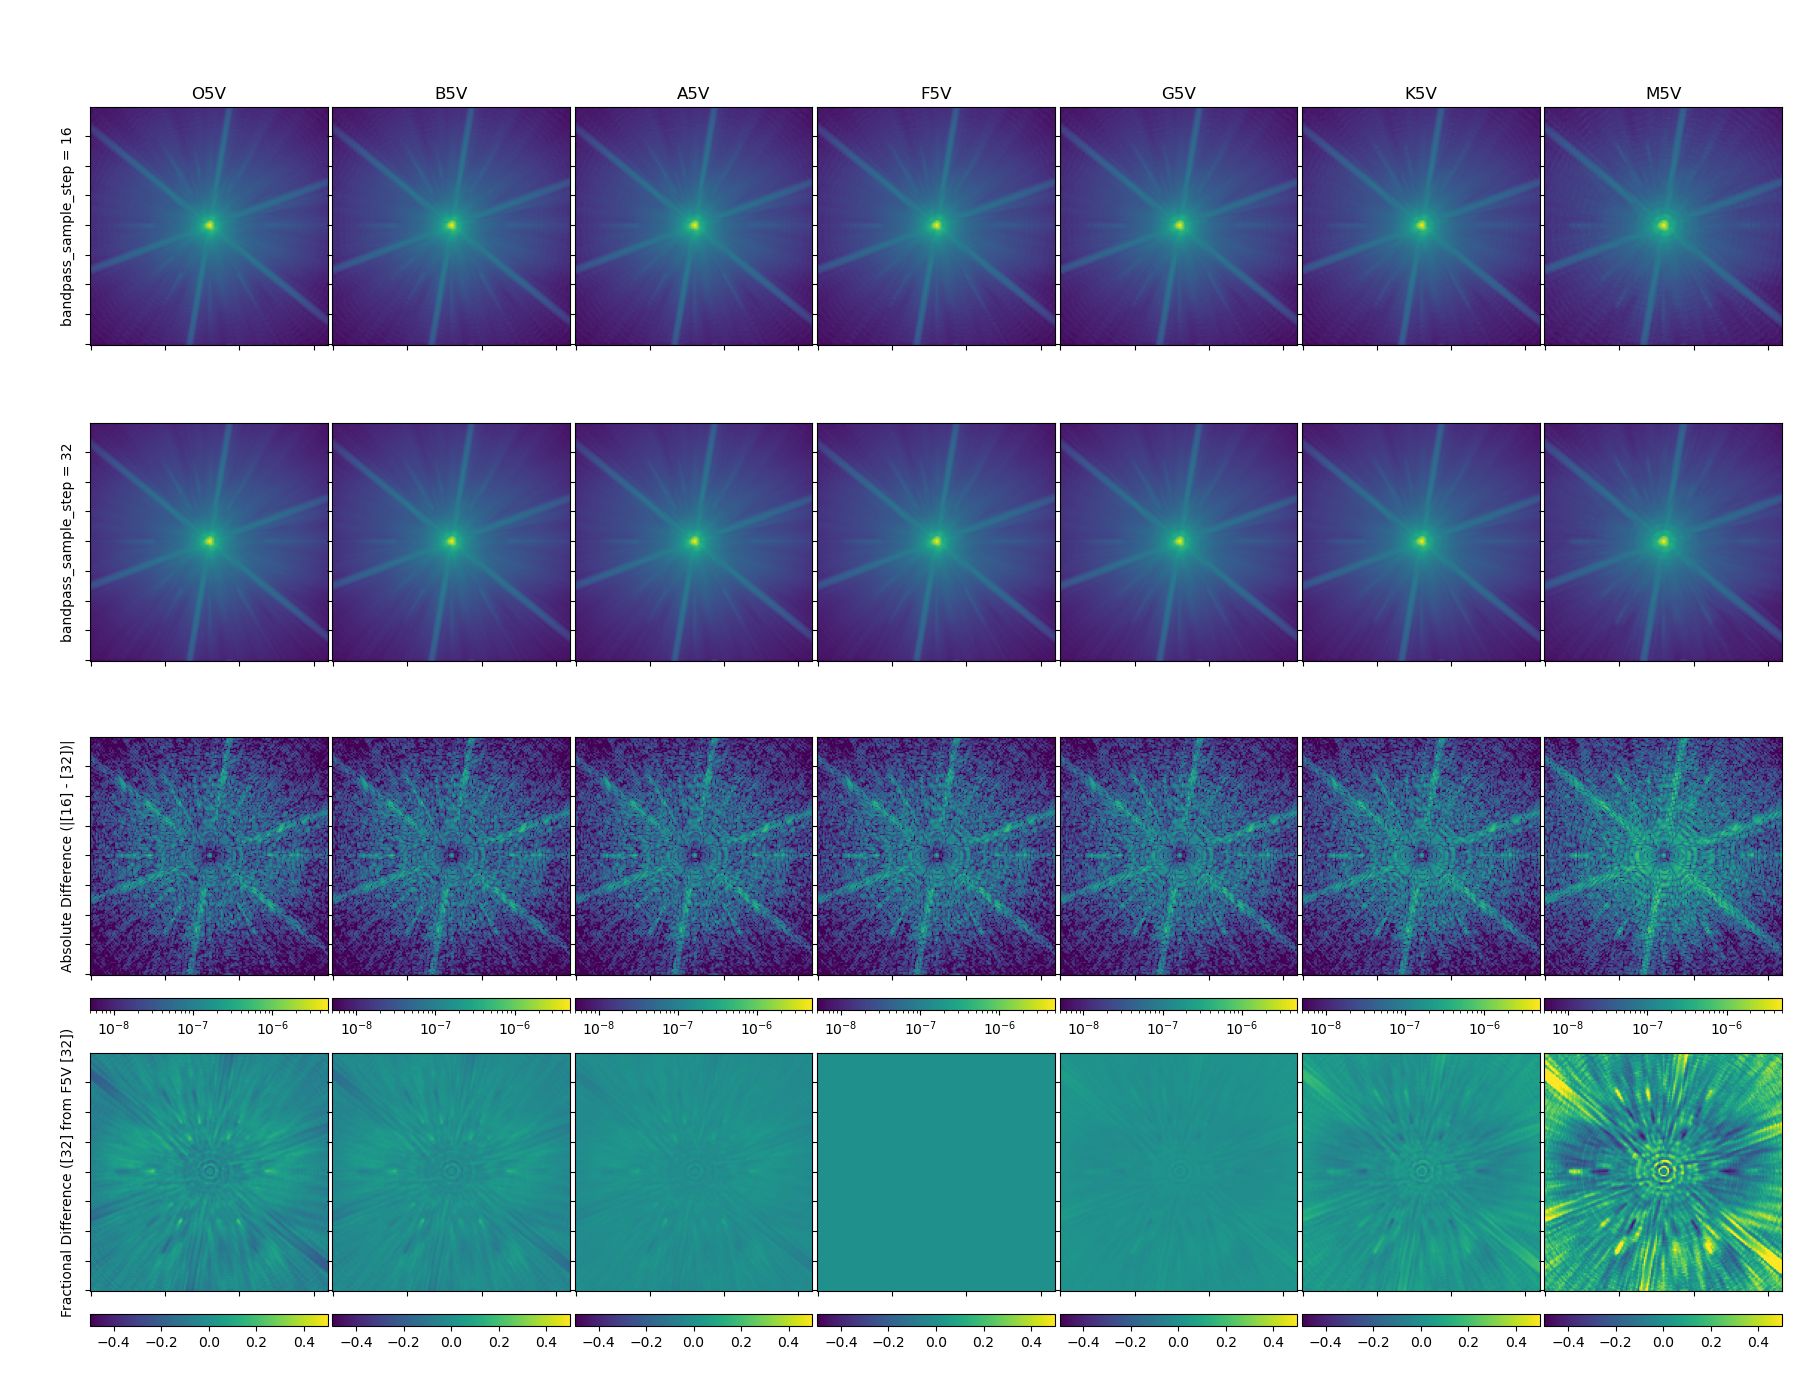
\includegraphics[width=\linewidth]{figures/bandpass_sample_step_dependency_of_psf.png}
    \caption{This figure illustrates the changes in the PSF as a function of the input spectra.
    From left to right the figure shows the PSFs and the differences in PSFs for OBAFGKM star
    spectra. Top: PSFs generated using 16 monochromatic basis PSFs. Second row: PSFs generated
    using 32 monochromatic basis PSFs. Third row: The difference between the first and second
    row. Bottom: The fractional difference between the respective PSFs from the PSF of the F
    star~(middle).}
    \label{fig:enter-label}
\end{figure}

%---------------------------------------------------------------------------------------------------
\subsection{Image Rendering}
%---------------------------------------------------------------------------------------------------
\textsc{Galsim} is the industrial standard for off-the-shelf rendering realistic simulated images.
We generate the PSFs with \textsc{PSFToolkit} and use \textsc{Galsim} to convolve with the stars
and galaxies from the input catalogues, and based on the WCS and pixel-scale defined in the image
header, see Section~\ref{sec:workflow}, \textsc{Galsim} render the source image postage stamps
which are then added to the base image. We only modify three configuration parameters from the
default values: (1)~\texttt{maximum\_fft\_size} is set to 40000 to allow larger FFT as there are
sufficient memory resources; the larger the convolution, the more accurate the contribution from
the tail of the PSFs can be modelled; (2)~\texttt{stepk\_minimum\_hlr} is set to 5, this sets the
k-space sampling where $\pi / \mathrm{step}_{k}$\footnote{step size in k-space} is at least multiple
of the \texttt{stepk\_minimum\_hlr} and the number of half-light-radius; (3) the 
\texttt{folding\_threshold} defines the tolerance of flux allowed to be folded back due to
insufficient FFT size. It is found from a set of look-up tables based on the flux ratio between the
peak flux and the sky background flux.

Another caveat is that when using \texttt{drawImage} method, \texttt{method} should be set to 
\texttt{"no\_pixel"} as this option is for externally provided PSF (real) images to avoid the
re-interpolation of the PSF which can lead to as much as 20\% discrepancy in the peak flux
of the PSF.

See Section~\ref{sec:shape_measurement} for further details on the treatment of pixel noise
and shape noise.
            
%---------------------------------------------------------------------------------------------------
\subsection{Simulation Volume}
%---------------------------------------------------------------------------------------------------

%---------------------------------------------------------------------------------------------------
\section{Shape Measurement}
%---------------------------------------------------------------------------------------------------
\label{sec:shape_measurement}

%---------------------------------------------------------------------------------------------------
\subsection{Shape Estimation methods}
%---------------------------------------------------------------------------------------------------
\subsubsection{LensMC}

\subsubsection{Metacal}

\subsection{Shape-noise cancellation}
We follow the description of shape-noise cancellation and the notation of Massey et al.\ (2007, STEP2).  
Intrinsic ellipticities are denoted $e_i^{\rm int}$, observed ellipticities $e_i^{\rm obs}$, 
and the true reduced shear by $\gamma$. A sample contains $N$ galaxies or, when shape-noise
cancellation is used, $N/2$ rotated pairs.

%--------------------------------------------------------------------
\subsubsection{Shot noise on the mean ellipticity}

Under the assumptions that intrinsic galaxy orientations are random
\begin{equation}
\langle e_i^{\rm int} \rangle = 0, 
\qquad 
\sigma_e^2 \equiv \langle (e_i^{\rm int})^2\rangle,
\end{equation}
the mean ellipticity of $N$ independent galaxies is given by
\begin{equation}
\bar e 
    = \frac{1}{N}\sum_{i=1}^N e_i^{\rm int}.
\end{equation}
Hence, the variance of ellipticity of N independent galaxies is,
\begin{equation}
{\rm Var}(\bar e)
    = \frac{{\rm Var}(e_i^{\rm int})}{N}
    = \frac{\langle (e_i^{\rm int})^2 \rangle 
            - \langle e_i^{\rm int} \rangle^2}{N}
    = \frac{\langle (e_i^{\rm int})^2\rangle}{N}.
\end{equation}
Therefore the one--sigma statistical (``shot noise'') uncertainty on the mean is
\begin{equation}
\sigma_{\bar e} 
    = \sqrt{\frac{\langle (e_i^{\rm int})^2 \rangle}{N}},
\end{equation}
\begin{equation}
\langle e^{\rm int} \rangle 
    = 0 \;\pm\; \sqrt{\frac{\langle (e_i^{\rm int})^2\rangle}{N}}.
\end{equation}
which is Equation~3 in STEP2.

%--------------------------------------------------------------------
\subsection*{Shot noise for the 90$^\circ$ rotated galaxy counterparts}
STEP2 forms a pair estimator using galaxies rotated by $90^\circ$.
Equation~(4) of the STEP2 paper defines the {\em pair mean} as
\begin{equation}
\tilde{\gamma}
    = \frac{e^{\rm obs,unrot} + e^{\rm obs,rot}}{2}.
\label{eq:ellipticiy_pair}
\end{equation}
%--------------------------------------------------------------------
STEP2 Equation (2) gives the exact shear transformation with the
$\ast$ denoting the complex conjugate:
\begin{equation}
e^{\rm obs} 
    = \frac{e^{\rm int} + \gamma}{1 + \gamma^\ast e^{\rm int}}.
\end{equation}
For $|\gamma|\ll1$, expand the denominator to first order:
\begin{equation}
\frac{1}{1 + \gamma^\ast e^{\rm int}}
    \approx 1 - \gamma^\ast e^{\rm int}.
\end{equation}
Thus,
\begin{equation}
e^{\rm obs}
    \approx 
    (e^{\rm int} + \gamma)
    (1 - \gamma^\ast e^{\rm int})
    =
    e^{\rm int} + \gamma
    - \gamma^\ast (e^{\rm int})^2
    + {\cal O}(\gamma^2).
\label{eq:eobs_expand}
\end{equation}
%--------------------------------------------------------------------
Rotation by $90^\circ$ sends $e^{\rm int} \rightarrow -\,e^{\rm int}$.  
This simplifies Equation~\eqref{eq:eobs_expand} to
\begin{equation}
e^{\rm obs,rot}
    \approx 
    - e^{\rm int}
    + \gamma
    - \gamma^\ast (e^{\rm int})^2
    + {\cal O}(\gamma^2).
\end{equation}

%--------------------------------------------------------------------
\subsubsection{Forming the pair estimator}
Insert the two expansions into Equation~\eqref{eq:ellipticiy_pair}:
\begin{equation}
\tilde{\gamma}
    =
    \frac{
        (e^{\rm int} + \gamma - \gamma^\ast (e^{\rm int})^2)
        +
        (- e^{\rm int} + \gamma - \gamma^\ast (e^{\rm int})^2)
    }{2}.
\end{equation}
The intrinsic ellipticity cancels:
\begin{equation}
e^{\rm int} + (-e^{\rm int}) = 0.
\end{equation}
Thus
\begin{equation}
\tilde{\gamma}
    \approx 
    \gamma
    - \gamma^\ast (e^{\rm int})^2.
\label{eq:gamma_tilde}
\end{equation}
The first term is the true shear;  
the second is the residual statistical noise after cancellation. Hence, the
noise on the true shear is
\begin{equation}
n_i \equiv - \gamma^\ast (e_i^{\rm int})^2,
\end{equation}
so that for one pair
\begin{equation}
\tilde{\gamma}_i = \gamma + n_i.
\end{equation}

%--------------------------------------------------------------------
\subsubsection{Variance of the mean over $N/2$ pairs}

There are $N/2$ independent rotated pairs.  Let $M = N/2$, the variance of the mean estimator is
\begin{equation}
{\rm Var}(\overline{\tilde\gamma})
    = \frac{{\rm Var}(n_i)}{M}.
\end{equation}
Since $\gamma$ is constant,
\begin{equation}
{\rm Var}(n_i)
    = |\gamma|^2 \;
      {\rm Var}\!\left((e_i^{\rm int})^2\right).
\end{equation}
The variance of the square is
\begin{equation}
{\rm Var}\!\left((e_i^{\rm int})^2\right)
 =
 \langle (e_i^{\rm int})^4\rangle
 -
 \langle (e_i^{\rm int})^2\rangle^2.
\end{equation}
Retaining only the leading term gives
\begin{equation}
{\rm Var}(n_i)
    \approx
    |\gamma|^2 \langle (e_i^{\rm int})^4\rangle.
\end{equation}
Therefore
\begin{equation}
{\rm Var}(\overline{\tilde{\gamma}})
    \approx
    \frac{|\gamma|^2 \langle (e_i^{\rm int})^4\rangle}{M}
    =
    \frac{2 |\gamma|^2 \langle (e_i^{\rm int})^4\rangle}{N}.
\end{equation}
The standard deviation is thus
\begin{equation}
\sigma_{\overline{\tilde{\gamma}}}
    =
    |\gamma|
    \sqrt{
        \frac{2\langle (e_i^{\rm int})^4\rangle}{N}
    }.
\end{equation}
STEP2 write this using their convention that 
$\langle (e_i^{\rm int})^4\rangle$ is defined per galaxy-pair ($M$ instead of $N$) such that
the above factor of $2$ is absorbed, leading to their Equation~(6) written as
\begin{equation}
{\rm SN\ error}
    \;\approx\;
    0 \;\pm\;
    \gamma \sqrt{\frac{\langle (e_i^{\rm int})^4\rangle}{2N}}.
\end{equation}

\subsection{Pixel-noise cancellation}

\subsection{Galaxy quadruplets -- combining shape-noise and pixel-noise cancellation}

Following the ideas introduced by early shear-testing studies 
(e.g.\ rotated-pair cancellation), consider a dataset in which each galaxy
is rendered in four versions:
a $0^\circ$ orientation with one pixel-noise realization,
a $0^\circ$ orientation with an inverted pixel-noise realization,
a $90^\circ$ orientation with the same pixel-noise realization,
and a $90^\circ$ orientation with the inverted noise realization.
The objective is to obtain a per-galaxy estimator that cancels the intrinsic
ellipticity at leading order while suppressing pixel-noise contributions.

\subsection*{i. Setup and notation}

Let $e^{\rm int}$ denote the intrinsic ellipticity component of a galaxy,
and let $s$ denote the deterministic shear response term for that galaxy.
In the weak-shear limit this is effectively the linear responsivity--shear
product ($P^\gamma\gamma$ in traditional notation).
For each of the four versions, define the measured ellipticities by
\begin{align}
e_A &= e^{\rm int} + s + \eta_A, \\
e_{A'} &= e^{\rm int} + s + \eta_{A'}, \\
e_B &= -\,e^{\rm int} + s + \eta_B, \\
e_{B'} &= -\,e^{\rm int} + s + \eta_{B'},
\end{align}
where subscripts $A$, $A'$, $B$, and $B'$ label respectively
the $(0^\circ,\ \text{noise})$, $(0^\circ,\ \text{inverted noise})$,
$(90^\circ,\ \text{noise})$, and $(90^\circ,\ \text{inverted noise})$
images.  
The terms $\eta_X$ represent the measurement and pixel-noise contributions,
with zero mean and covariances to be specified below.
The $90^\circ$ rotation flips the sign of the intrinsic ellipticity component.

\subsection*{ii. Quadruplet estimator and cancellation of intrinsic shape}

Define the per-galaxy quadruplet mean as
\begin{equation}
\bar e \equiv \frac{e_A + e_{A'} + e_B + e_{B'}}{4}.
\end{equation}
Substituting the expressions above gives
\begin{align}
\bar e
&= \frac{1}{4}
   \big[(e^{\rm int}+s+\eta_A)
      + (e^{\rm int}+s+\eta_{A'})
      + (-e^{\rm int}+s+\eta_B)
      + (-e^{\rm int}+s+\eta_{B'})\big] \\
&= s + \frac{\eta_A + \eta_{A'} + \eta_B + \eta_{B'}}{4}.
\end{align}
Thus the intrinsic ellipticity cancels exactly to first order, leaving a
shear response term $s$ plus a noise term defined by the average over the
four pixel-noise contributions.

\subsection*{iii. General covariance of the quadruplet mean}

Let $C_X=\mathrm{Cov}(\eta_X)$ and 
$C_{XY}=\mathrm{Cov}(\eta_X,\eta_Y)$ be the $2\times2$ covariance
and cross-covariance matrices for the noise terms of the
ellipticity components.
The covariance matrix of $\bar e$ for a single quadruplet is then
\begin{align}
\mathrm{Cov}(\bar e)
&= \mathrm{Cov}\!\left(\frac{\eta_A + \eta_{A'} + \eta_B + \eta_{B'}}{4}\right) \\
&= \frac{1}{16}\big(C_A + C_{A'} + C_B + C_{B'} 
    + C_{AA'} + C_{A'A} + C_{AB} + C_{BA}
    + C_{AB'} + C_{B'A} \nonumber \\
&\qquad\qquad 
    + C_{A'B} + C_{BA'} + C_{A'B'} + C_{B'A'}
    + C_{BB'} + C_{B'B}\big).
\end{align}
This expression is exact and incorporates all correlations between
noise realizations across the four images.

When all four noise fields have identical covariance,
$C_A=C_{A'}=C_B=C_{B'}\equiv C$,
the diagonal contributions reduce to $4C$, and the remainder is determined
entirely by the twelve cross-covariance matrices.

\subsection*{iv. Scalar per-component form under equal variances}

A common simplification is a scalar treatment per ellipticity component,
assuming equal per-component variances,
\begin{equation}
\mathrm{Var}(\eta_X)=\sigma^2 \qquad
\text{for all } X\in\{A,A',B,B'\}.
\end{equation}
Define the per-component correlation coefficients
\begin{align}
\rho_{\rm inv} &= \mathrm{Corr}(\eta_A,\eta_{A'}),\\
\rho_{\rm rot} &= \mathrm{Corr}(\eta_A,\eta_{B}), \\
\rho_{\rm rot\_inv} &= \mathrm{Corr}(\eta_A,\eta_{B'}).
\end{align}
By symmetry, the remaining correlations take the same or sign-reflected
values depending on the structure of the noise inversion.

Under these assumptions, the variance per component of the quadruplet mean is
\begin{equation}
\sigma_{\rm quad}^2
= \frac{\sigma^2}{4}
  \big(1 + \rho_{\rm inv} + \rho_{\rm rot} + \rho_{\rm rot\_inv}\big).
\end{equation}
If the inverted pixel-noise field is perfectly anticorrelated with the
uninverted version (an exact Gaussian negation), then
$\rho_{\rm inv}=-1$ and the corresponding cross-covariances cancel part or all 
of the diagonal terms.
In that case the measurement noise can be suppressed dramatically or even
eliminated provided the ellipticity measurement algorithm is sufficiently
linear.
For Poisson antithetic constructions, $\rho_{\rm inv}$ is typically negative
but strictly greater than $-1$, providing partial but not complete cancellation.

\subsection*{v. Residual intrinsic--shear coupling}

Although the intrinsic ellipticity cancels at leading order under the
$0^\circ$/$90^\circ$ rotation, higher-order terms in the shear transformation
produce a residual proportional to $(e^{\rm int})^2$.
Expanding the shear transformation to first order in shear and second order in
intrinsic ellipticity yields, for a given galaxy,
\begin{equation}
\bar e \approx s - \gamma^\ast (e^{\rm int})^2 + \text{noise},
\end{equation}
where $\gamma$ is the reduced shear and the term
$\gamma^\ast (e^{\rm int})^2$ is stochastic due to the intrinsic ellipticity.
Let $n_i = -\gamma^\ast (e_i^{\rm int})^2$ denote this residual term for the
$i$-th galaxy.
The variance of $n_i$ is
\begin{equation}
\mathrm{Var}(n_i)
= |\gamma|^2\,\mathrm{Var}\!\left((e^{\rm int})^2\right)
\approx |\gamma|^2\langle (e^{\rm int})^4\rangle,
\end{equation}
where the approximation drops the term
$\langle (e^{\rm int})^2\rangle^2$, which is numerically subdominant for
typical galaxy ellipticity distributions.

Let $N_{\rm quad}$ be the number of independent quadruplets in the dataset.
Since the quadruplets are independent,
\begin{equation}
\mathrm{Var}_{\rm intr}(\overline{n})
= \frac{|\gamma|^2\langle (e^{\rm int})^4\rangle}{N_{\rm quad}}.
\end{equation}

\subsection*{vi. Total variance of the shear estimator from quadruplets}

Suppose a shear estimator $\hat\gamma$ is formed from the sample average
of $\bar e$ (after metacalibration, if needed).
The two statistically independent contributions to the variance of
$\hat\gamma$ are the measurement and pixel-noise contribution from the
quadruplet average and the intrinsic ellipticity residual.
The resulting per-component variance is
\begin{equation}
\mathrm{Var}(\hat\gamma)
\approx
\frac{\sigma_{\rm quad}^2}{N_{\rm quad}}
+
\frac{|\gamma|^2\langle (e^{\rm int})^4\rangle}{N_{\rm quad}},
\end{equation}
where $\sigma_{\rm quad}^2$ is given above and
$N_{\rm quad}$ is the number of independent quadruplets.
The first term represents the residual measurement and pixel-noise after
noise inversion and rotation, while the second term reflects the 
second-order intrinsic-shear coupling that remains even when measurement 
noise is perfectly cancelled.


The quadruplet construction eliminates the intrinsic ellipticity at leading
order and can substantially suppress or eliminate pixel noise depending on
the correlation structure of the inverted noise fields.
The residual variance of the shear estimator consists of a measurement-noise
term proportional to the pixel-noise covariance and an intrinsic--shear
term proportional to $|\gamma|^2\langle (e^{\rm int})^4\rangle$.
Both contributions scale inversely with the number of independent quadruplets.


%---------------------------------------------------------------------------------------------------
\section{Workflow (Pipeline Description)}
\label{sec:workflow}
The workflow of the sensitivity test is divided into three pipeline runs, each runs several
executables that parallelise the tasks differently to use the computing resources optimally. The
first step of the workflow is the most computationally heavy one, it simulates the noiseless images;
the second one applies backgrounds and noises, and measures the shapes to produce the raw catalogues;
the third one performs calibration and computes the biases. Depending on the parameters of the
sensitivity test to perform, in some cases, the noiseless images can be reused.

\subsection{Noiseless Image Simulation}

The following programs are run in the execution of this pipeline:

\begin{itemize}
    \item \texttt{SHE\_SENS\_GenerateQuadNumList}
    \item \texttt{SHE\_SENS\_CreateNoiselessMockQuadImage}
\end{itemize}

\subsubsection{High-level description of this pipeline}

\underline{Prerequisite}
\begin{enumerate}
    \item \texttt{dpdVISCalibratedQuadFrame} from the Euclid Archive System~(EAS)
    \item SIM True Universe star catalogues and Flagship galaxy catalogues
\end{enumerate}

\noindent \underline{Pipeline}
\begin{enumerate}
    \item Execute \texttt{SHE\_SENS\_GenerateQuadNumList} to enable parallelisation into 144 concurrent processes (each processor handles one \texttt{quad\_num}). This is an intermediate executable used in runtime so it is not described further in the I/O port descriptions.
    \item Execute \texttt{SHE\_SENS\_CreateNoiselessMockQuadImage} to:
        \begin{itemize}
            \item Take the \texttt{dpdVISCalibratedQuadFrame} to get the detector properties and the WCSs.
            \item Load the star and galaxy catalogues overlapping the footprint described by the WCSs.
            \item Use \textsc{PSFToolkit} to generate monochromatic basis set for each quadrant
            \item Use \textsc{PSFToolkit} to generate SED-dependent PSFs
            \item Use \textsc{Galsim} to convolve the PSFs with the star and galaxy profiles (where the operations for the galaxies are embarrassingly parallelised, we use four cores for this step\footnote{See more in \url{https://euclid.roe.ac.uk/projects/sgsshear/wiki/20241007_Monday_Meeting}})
            \item Repeat with a 90 degrees rotation angle for the galaxy profiles to create a set of the twin images for shape-noise cancellation
        \end{itemize}
\end{enumerate}

\subsubsection{I/O Ports}

\tikzstyle{every node}=[font=\scriptsize]
\begin{center}
\begin{tikzpicture}[
  node distance=0.15cm,
  smallbox/.style={draw, rounded corners, minimum height=0.8cm, text width=7.5cm, align=center},
  smallcircle/.style={draw, circle, minimum size=0.8cm, text width=7.5cm, align=center},
  bigellipse/.style={draw, ellipse, minimum height=1.5cm, align=center},
  arrow/.style={-Latex},
]

  % Input items
  \node (input1) [smallbox] {\texttt{input\_vis\_quadframe} (1)\\DpdVisCalibratedQuadFrame};
  %\node (input2) [smallbox, below=of input1] {Input 2};
  
  % Process box
  \node (pipeline) [bigellipse, below=of input1, yshift=-0.25cm] {\texttt{PipScript\_SHE\_SENS\_Noiseless\_Simulation}};

  % Output items
  \node (output1) [smallbox, below=of pipeline, yshift=-0.25cm] {\texttt{merged\_psfmodelimages} (1)\\DpdShePsfModelImage};
  \node (output2) [smallbox, below=of output1] {\texttt{merged\_psfmodelimages\_lst} (1)\\DpdShePsfModelImage};
  \node (output3) [smallbox, below=of output2] {\texttt{h5\_noiseless\_quad\_image} (1..144)\\DpdVisCalibratedQuadFrame};
  \node (output4) [smallbox, below=of output3] {\texttt{h5\_noiseless\_quad\_image\_rot90} (1..144)\\DpdVisCalibratedQuadFrame};

  % Define the number of input and output items
  \def\M{1} % Number of input items
  \def\N{4} % Number of output items

  % Connect input items to the pipeline ellipse
  \foreach \i in {1,...,\M} {
    \draw [arrow] (input\i.west) -- ++(-3.0cm, 0) |- ([xshift=-0.5cm]pipeline.west) -- (pipeline.west); 
  }
  
  % Connect the pipeline ellipse to output items (from right)
  \foreach \i in {1,...,\N} {
    \draw [arrow] (pipeline.east) -- ++(2.0cm, 0) |- (output\i.east);
  }

\end{tikzpicture}
\end{center}


\subsubsection{Port Descriptions}
Input:

\begin{enumerate}
    \item \texttt{input\_vis\_quadframe\_dpd}: A data product of a calibrated quadrant-based full frame VIS image.
\end{enumerate}

\noindent Output:

\begin{enumerate}
    \item \texttt{merged\_psfmodelimages}: A data product of a h5 file storing PSFs used in the image simulation (for MetaCal).
    \item \texttt{merged\_psfmodelimages\_lst}: A listfile of four \texttt{merged\_psfmodelimages} (for LensMC).
    \item \texttt{h5\_noiseless\_quad\_image}: A listfile of 144 noiseless simulated quadrant images, in h5 formats.
    \item \texttt{h5\_noiseless\_quad\_image\_rot90}: A listfile of 144 noiseless simulated quadrant images with galaxies rotated by 90 degrees for shape-noise cancellation, in h5 formats.
\end{enumerate}

\subsubsection{Other Requirements}

The configuration files of \textsc{PSFToolkit} and \textsc{SENS} should be updated inside the \texttt{auxdir}, or provided in the \texttt{isf} file or pipeline script, with particular importance are the folder locations of the star and galaxy catalogues.

\subsubsection{Operational constraints}

\noindent EDEN: Eden-3.1\\
\noindent Data Model: 10.1.2\\
\noindent Workdir size (est.): 100\,GB

\subsubsection{Hardware configuration and related performances}

\begin{table}[]
    \centering
    \begin{tabular}{|l|c|c|c|}
         \hline
         Processing Element                               & Cores & RAM (GB) & Walltime (hours) \\
         \hline
         \texttt{SHE\_SENS\_GenerateQuadNumList}          & 1     & 0.1      & 0.01 \\
         \texttt{SHE\_SENS\_CreateNoiselessMockQuadImage} & 576   & 64       & 4  \\
         \hline
    \end{tabular}
    \caption{Caption}
    \label{tab:my_label}
\end{table}

\noindent Normal termination
The SENS simulation pipeline is managed by the Elements \texttt{E-Run} command so in the case of normal termination, the standard output of the \texttt{E-Run} command is expected.


%---------------------------------------------------------------------------------------------------
\subsection{Noisy Image and Shape Measurement}

The following programs are run in the execution of this pipeline:

\begin{itemize}
    \item \texttt{SHE\_SENS\_CreateFourNoiseRealisationMockQuadImages}
    \item \texttt{SHE\_SENS\_JoinInputCatalogues}
    \item \texttt{SHE\_SENS\_CreatePHZCatalogue}
    \item \texttt{SHE\_MetaCal\_EstimateShear}
    \item \texttt{SHE\_MetaCal\_StackRawMeasurements}
    \item \texttt{SHE\_LensMC\_EstimateShear}
    \item \texttt{SHE\_CTE\_ShearEstimatesMerge}
    \item \texttt{SHE\_SENS\_CreateFullFrameImage}
\end{itemize}

\subsubsection{High-level description of this pipeline}

\begin{enumerate}
    \item Execute \texttt{SHE\_SENS\_CreateFourNoiseRealisationMockQuadImages} to
        \begin{itemize}
            \item Add read noise and shot noise to each frame 4 times for each rotation angle and for each of the `positive' and `negative' noise [total number of frames becomes 18 ($4 \times 2 \times 2$ noisy and 2 noiseless)]
            \item Generate segmentation maps and segmentation catalogues using the configuration file available from MER to run \texttt{SourceXtractorPlusPlus}
            \item Left join segmentation catalogue onto the input catalogues
        \end{itemize}
    \item Execute \texttt{SHE\_SENS\_JoinInputCatalogues} to merge quadrant-based input catalogues and \texttt{PSFModelImages} to per full-frame
    \item Execute \texttt{SHE\_SENS\_CreatePHZCatalogue} to generate a PHZ catalogue based on the merged input catalogue and PHZ tomographic bins
    \item Execute \texttt{SHE\_SENS\_CreateFullFrameImage} to generate a quicklook PNG image of the full-frame image.
    \item To get shapes from \texttt{MetaCal}, execute \texttt{SHE\_MetaCal\_EstimateShear} to measure galaxy shapes; and \texttt{SHE\_MetaCal\_StackRawMeasurements} to produce a raw catalogue per full-frame
    \item To get shapes from \texttt{LensMC}, execute \texttt{SHE\_LensMC\_EstimateShear} to measure galaxy shapes; and \texttt{SHE\_CTE\_ShearEstimatesMerge} to produce a raw catalogue per full-frame
\end{enumerate}


\subsubsection{I/O Ports}

\tikzstyle{every node}=[font=\scriptsize]
\begin{center}
\begin{tikzpicture}[
  node distance=0.15cm,
  smallbox/.style={draw, rounded corners, minimum height=0.8cm, text width=9.0cm, align=center},
  smallcircle/.style={draw, circle, minimum size=0.8cm, text width=8.0cm, align=center},
  bigellipse/.style={draw, ellipse, minimum height=1.5cm, align=center},
  arrow/.style={-Latex},
]

  % Input items
  \node (input1) [smallbox] {\texttt{h5\_noiseless\_quad\_image\_filelist} (1..144)\\DpdVisCalibratedQuadFrame};
  \node (input2) [smallbox, below=of input1] {\texttt{h5\_noiseless\_quad\_image\_rot90\_filelist} (1..144)\\DpdVisCalibratedQuadFrame};
  \node (input3) [smallbox, below=of input2] {\texttt{input\_vis\_quadframe} (1)\\DpdVisCalibratedQuadFrame};
  \node (input4) [smallbox, below=of input3] {\texttt{tom\_bin\_dpd} (1)\\DpdTomographicBins};
  \node (input5) [smallbox, below=of input4] {\texttt{psf\_model\_images\_lst} (1..144)\\PSFModelImages};
  
  % Process box
  \node (pipeline) [bigellipse, below=of input5, yshift=-0.25cm] {\texttt{PipScript\_SHE\_SENS\_Add\_Noise\_And\_Estimate\_Shear}};

  % Output items
  \node (output1) [smallbox, below=of pipeline, yshift=-0.25cm] {\texttt{she\_metacal\_unweighted\_measurements} (1..144)\\SheMetaCalRawCatalog};
  \node (output2) [smallbox, below=of output1] {\texttt{she\_lensmc\_uncorrected\_shear\_estimates\_product} (1..144)\\DpdSheLensMcRawCatalog};
  \node (output3) [smallbox, below=of output2] {\texttt{she\_lensmc\_chains} (1..144)\\DpdSheLensMcChains};
  \node (output4) [smallbox, below=of output3] {\texttt{she\_metacal\_unweighted\_measurements\_rot90} (1..144)\\SheMetaCalRawCatalog};
  \node (output5) [smallbox, below=of output4] {\texttt{she\_lensmc\_uncorrected\_shear\_estimates\_product\_rot90} (1..144)\\DpdSheLensMcRawCatalog};
  \node (output6) [smallbox, below=of output5] {\texttt{she\_lensmc\_chains\_rot90} (1..144)\\DpdSheLensMcChains};
  \node (output7) [smallbox, below=of output6] {\texttt{input\_galaxy\_catalogs\_filepath} (1)\\DpdGalaxyCatalogProduct};
  \node (output8) [smallbox, below=of output7] {\texttt{input\_galaxy\_catalogs\_filepath\_lst} (1)\\DpdGalaxyCatalogProduct};
  \node (output9) [smallbox, below=of output8] {\texttt{input\_catalogs\_filepath} (1)\\DpdGalaxyCatalogProduct};
  \node (output10) [smallbox, below=of output9] {\texttt{input\_catalogs\_filepath\_lst} (1)\\DpdGalaxyCatalogProduct};
  \node (output11) [smallbox, below=of output10] {\texttt{mer\_catalogs\_filepath} (1)\\DpdMerFinalCatalog};
  \node (output12) [smallbox, below=of output11] {\texttt{phz\_catalogs\_filepath} (1)\\DpdPhzPfOutputCatalog};
  \node (output13) [smallbox, below=of output12] {\texttt{fullframe\_image\_filepath} (1)\\DpdSheIntermediateGeneral};
  \node (output14) [smallbox, below=of output13] {\texttt{fullframe\_image\_rot90\_filepath} (1)\\DpdSheIntermediateGeneral};
    
  % Define the number of input and output items
  \def\M{5} % Number of input items
  \def\N{14} % Number of output items

  % Connect input items to the pipeline ellipse
  \foreach \i in {1,...,\M} {
    \draw [arrow] (input\i.west) -- ++(-3.0cm, 0) |- ([xshift=-0.5cm]pipeline.west) -- (pipeline.west); 
  }
  
  % Connect the pipeline ellipse to output items (from right)
  \foreach \i in {1,...,\N} {
    \draw [arrow] (pipeline.east) -- ++(2.0cm, 0) |- (output\i.east);
  }

\end{tikzpicture}
\end{center}

\subsubsection{Port Descriptions}
Input:

\begin{enumerate}
    \item \texttt{h5\_noiseless\_quad\_image\_filelist}: A listfile of the per quadrant noiseless image in h5 format storing a complete \texttt{QuadImage}, a proprietary \textsc{SHE\_SENS} object, including all the metadata and auxiliary data that are necessary to continue the simulation.
    \item \texttt{h5\_noiseless\_quad\_image\_rot90\_filelist}: The same as above for the shape-noise cancellation galaxies rotated by 90 degrees.
    \item \texttt{input\_vis\_quadframe\_dpd}: A data product of a calibrated quadrant-based full frame VIS image. This should be the same one used in the noiseless image simulation.
    \item \texttt{tom\_bin\_dpd}: A PHZ data product describing the tomographic bin edges.
    \item \texttt{psf\_model\_images\_lst}: A listfile of \texttt{PSFModelImages} from the noiseless image simulation, it has the same length as the input star and galaxy catalogues combined.
\end{enumerate}

\noindent Output:

\begin{enumerate}
    \item \texttt{she\_metacal\_unweighted\_measurements}: The raw \textsc{MetaCal} measurements.
    \item \texttt{she\_lensmc\_uncorrected\_shear\_estimates\_product}: The raw \textsc{LensMC} measurements.
    \item \texttt{she\_lensmc\_chains}: The MCMC chains used by \textsc{LensMC}.
    \item \texttt{she\_metacal\_unweighted\_measurements\_rot90}: The same as above with the shape-noise cancellation galaxies rotated by 90 degrees.
    \item \texttt{she\_lensmc\_uncorrected\_shear\_estimates\_product\_rot90}: The same as above with the shape-noise cancellation galaxies rotated by 90 degrees.
    \item \texttt{she\_lensmc\_chains\_rot90}: The same as above with the shape-noise cancellation galaxies rotated by 90 degrees.
    \item \texttt{input\_galaxy\_catalogs\_filepath}: The catalogue containing all the galaxies with the centroid in that quad image.
    \item \texttt{input\_galaxy\_catalogs\_filepath\_lst}: The format for the input port of \textsc{LensMC}.
    \item \texttt{input\_catalogs\_filepath}: The catalogue containing all the stars and galaxies with the centroid in that quad image.
    \item \texttt{input\_catalogs\_filepath\_lst}: The format for the input port of \textsc{LensMC} (should \textsc{LensMC} measures stars in the future).
    \item \texttt{mer\_catalogs\_filepath}: The MER catalogue produced using the segmentation map from \textsc{SourceXtractorPlusPlus}.
    \item \texttt{phz\_catalogs\_filepath}: A minimal PHZ catalogue with a column of object ID and a column of tomographic bin ID.
    \item \texttt{fullframe\_image\_filepath}: A full frame PNG image.
    \item \texttt{fullframe\_image\_rot90\_filepath}: A full frame PNG image with the shape-noise cancellation galaxies rotated by 90 degrees.
\end{enumerate}

\subsubsection{Other Requirements}

The configuration files of \textsc{SENS} should be updated inside the \texttt{auxdir}, or provided in the \texttt{isf} file or pipeline script.
\textsc{SourceXtractorPlusPlus} is called in a subprocess when executing \texttt{SHE\_SENS\_CreateFourNoiseRealisationMockQuadImages}. 

\subsubsection{Operational constraints}

\noindent EDEN: Eden-3.1\\
\noindent Data Model: 10.1.2\\
\noindent Workdir size (est.): 1000\,GB

\subsubsection{Hardware configuration and related performances}

\begin{table}[]
    \centering
    \begin{tabular}{|l|c|c|c|}
         \hline
         Processing Element                                           & Cores & RAM (GB) & Walltime (hours) \\
         \hline
         \texttt{SHE\_SENS\_CreateFourNoiseRealisationMockQuadImages} & 144   & 1.0      & 0.50 \\
         \texttt{SHE\_SENS\_JoinInputCatalogues}                      & 1     & 2.0      & 0.50 \\
         \texttt{SHE\_SENS\_CreatePHZCatalogue}                       & 1     & 2.0      & 0.50 \\
         \texttt{SHE\_SENS\_CreateFullFrameImage}                     & 1     & 5.0      & 0.50 \\
         \texttt{SHE\_MetaCal\_EstimateShear}                         & 144   & 2.5      & 1.00 \\
         \texttt{SHE\_MetaCal\_StackRawMeasurements}                  & 1152  & 2.5      & 1.00 \\
         \texttt{SHE\_LensMC\_EstimateShear}                          & 144   & 2.0      & 4.00 \\
         \texttt{SHE\_CTE\_ShearEstimatesMerge}                       & 4     & 4.0      & 1.00 \\
         \hline
    \end{tabular}
    \caption{Caption}
    \label{tab:my_label}
\end{table}

%---------------------------------------------------------------------------------------------------
\subsection{MetaCal Bias Measurement}






The following programs are run in the execution of this pipeline:

\begin{itemize}
    \item \texttt{SHE\_SENS\_JoinListFiles}
    \item \texttt{SHE\_CTE\_UpdateShapeNoise}
    \item \texttt{SHE\_MetaCal\_Calibrate}
    \item \texttt{SHE\_Calibration\_MeasureBias}
\end{itemize}

\subsubsection{High-level description of this pipeline}

\begin{enumerate}
    \item Execute \texttt{SHE\_SENS\_JoinListFiles} to join the listfiles of the shape-noise cancellation pairs of data for the MER catalogues, PHZ catalogues and the input galaxy catalogues.
    \item Execute \texttt{SHE\_MetaCal\_Calibrate} to metacalibrate the raw measurements to produce
    the \texttt{metacal\_final\_catalogue}.
    \item Execute \texttt{SHE\_CTE\_UpdateShapeNoise} to update the noise of the measurement to include shape-noise.
    \item Execute \texttt{SHE\_Calibration\_MeasureBias} to compute $m_{11}$, $m_{12}$, $m_{21}$, $m_{22}$, $c_{1}$ and $c_{2}$.
\end{enumerate}

\subsubsection{I/O Ports}

\tikzstyle{every node}=[font=\scriptsize]
\begin{center}
\begin{tikzpicture}[
  node distance=0.15cm,
  smallbox/.style={draw, rounded corners, minimum height=0.8cm, text width=7.5cm, align=center},
  smallcircle/.style={draw, circle, minimum size=0.8cm, text width=7.5cm, align=center},
  bigellipse/.style={draw, ellipse, minimum height=1.5cm, align=center},
  arrow/.style={-Latex},
]

  % Input items
  \node (input1) [smallbox] {\texttt{metacal\_raw\_catalogs\_listfile} (N)\\SheMetaCalRawCatalog};
  \node (input2) [smallbox, below=of input1] {\texttt{metacal\_raw\_catalogs\_rot90\_listfile} (N)\\SheMetaCalRawCatalog};
  \node (input3) [smallbox, below=of input2] {\texttt{sim\_tu\_catalogs} (N)\\DpdGalaxyCatalogProduct};
  \node (input4) [smallbox, below=of input3] {\texttt{mer\_final\_catalogs} (N)\\DpdMerFinalCatalog};
  \node (input5) [smallbox, below=of input4] {\texttt{phz\_catalogs} (N)\\DpdPhzPfOutputCatalog};
  \node (input6) [smallbox, below=of input5] {\texttt{metacal\_shape\_noise} (1)\\DpdSheIntermediateGeneral};
  
  % Process box
  \node (pipeline) [bigellipse, below=of input6, yshift=-0.25cm] {\texttt{PipScript\_SHE\_SENS\_MetaCal\_Calibration}};

  % Output items
  \node (output1) [smallbox, below=of pipeline, yshift=-0.25cm] {\texttt{metacal\_final\_catalogs\_listfile} (1)\\SheMetaCalFinalCatalog};
  \node (output2) [smallbox, below=of output1] {\texttt{bias\_measurements} (1)\\DpdSheBiasParams};

  % Define the number of input and output items
  \def\M{6} % Number of input items
  \def\N{2} % Number of output items

  % Connect input items to the pipeline ellipse
  \foreach \i in {1,...,\M} {
    \draw [arrow] (input\i.west) -- ++(-3.0cm, 0) |- ([xshift=-0.5cm]pipeline.west) -- (pipeline.west); 
  }
  
  % Connect the pipeline ellipse to output items (from right)
  \foreach \i in {1,...,\N} {
    \draw [arrow] (pipeline.east) -- ++(2.0cm, 0) |- (output\i.east);
  }

\end{tikzpicture}
\end{center}


\subsubsection{Port Descriptions}
Input:

\begin{enumerate}
    \item \texttt{metacal\_raw\_catalogs\_listfile}: The raw \textsc{MetaCal} measurements.
    \item \texttt{metacal\_raw\_catalogs\_rot90\_listfile}: The raw \textsc{MetaCal} measurements for the shape-noise cancellation set of galaxies rotated by 90 degrees.
    \item \texttt{sim\_tu\_catalogs}: The catalogue containing all the galaxies with the centroid in that full-frame image.
    \item \texttt{mer\_final\_catalogs}: The MER catalogue produced using the segmentation map from \textsc{SourceXtractorPlusPlus}.
    \item \texttt{phz\_catalogs}: A minimal PHZ catalogue with a column of object ID and a column of tomographic bin ID.
    \item \texttt{metacal\_shape\_noise}: Intrinsic shape-noise error from using \textsc{MetaCal}.
\end{enumerate}

\noindent Output:

\begin{enumerate}
    \item \texttt{metacal\_final\_catalogs\_listfile}: The final metacalibrated \textsc{MetaCal} measurements.
    \item \texttt{bias\_measurements}: The $m$ and $c$ biases.
\end{enumerate}

\subsubsection{Other Requirements}

The configuration files of \textsc{PSFToolkit} and \textsc{SENS} should be updated inside the \texttt{auxdir}, or provided in the \texttt{isf} file or pipeline script, with particular importance are the folder locations of the star and galaxy catalogues.

\subsubsection{Operational constraints}

\noindent EDEN: Eden-3.1\\
\noindent Data Model: 10.1.2\\
\noindent Workdir size (est.): 2\,GB

\subsubsection{Hardware configuration and related performances}

\begin{table}[]
    \centering
    \begin{tabular}{|l|c|c|c|}
         \hline
         Processing Element                     & Cores & RAM (GB) & Walltime (hours) \\
         \hline
         \texttt{SHE\_SENS\_JoinListFiles}      & 1     & 0.1      & 0.1 \\
         \texttt{SHE\_CTE\_UpdateShapeNoise}    & 1     & 4        & 0.1 \\
         \texttt{SHE\_MetaCal\_Calibrate}       & 1     & 8        & 0.1 \\
         \texttt{SHE\_Calibration\_MeasureBias} & 1     & 8        & 0.1 \\
         
         \hline
    \end{tabular}
    \caption{Caption}
    \label{tab:my_label}
\end{table}

\noindent Normal termination
The SENS simulation pipeline is managed by the Elements \texttt{E-Run} command so in the case of normal termination, the standard output of the \texttt{E-Run} command is expected.










%---------------------------------------------------------------------------------------------------
\subsection{LensMC Bias Measurement}
\begin{enumerate}
    \item Execute \texttt{SHE\_Calibration\_MeasureBias} to compute $m_{11}$, $m_{12}$, $m_{21}$,
    $m_{22}$, $c_{1}$ and $c_{2}$
\end{enumerate}



%---------------------------------------------------------------------------------------------------
\section{Results}
\label{sec:results}
%---------------------------------------------------------------------------------------------------

\end{document}


